\chapter{Recuperação de imagens baseada em conteúdo}

Os primeiros trabalhos sobre recuperação de imagens são datados do final da década de 1970. Em 1979, uma conferência sobre \textit{Database Techniques for Pictorial Applications} (numa tradução livre "Técnicas de banco de dados para aplicações com imagens") foi realizada em Florência, Itália. Desde então, o potencial de técnicas de gerenciamento de banco de dados de imagens atraíu a atenção dos pesquisadores.

As primeiras técnicas não foram baseadas em características visuais e sim em anotações textuais das imagens. Em outras palavras, as imagens eram primeiro descritas textualmente, para então serem recuperadas usando busca baseada em texto dos sistemas de gerenciamente de banco de dados tradicionais. Através das descrições textuais, as imagens podem ser organizadas por tópicos ou classes hierárquicas para facilitar a busca através de requisições usando expressões lógicas. Entretanto, como a geração automática de descrições para imagens diversas é uma tarefa quase impossível, a maioria dos sistemas de recuperação baseados em imagem requer que as descrições sejam feitas manualmente. Obviamente, fazer anotações manualmente sobre uma imagem é uma tarefa difícil e onerosa para grandes bancos de dados de imagens, além de ser geralmente subjetiva, sensível ao contexto e incompleta \cite{feng-chapter}.

O objetivo dos sistemas de recuperação de imagens baseada em conteúdo - CBIR (content based image retrieval) - é buscar em um banco de imagens as imagens mais relevantes relativas a uma requisição visual. Dessa forma eliminando a necessidade de descrições textuais manuais e tornando a busca mais eficiente e menos subjetiva.

Num sistema CBIR típico, o conteúdo visual relevante das imagens no banco de imagens é extraído e armazenado como um vetor de características. Para realizar a recuperação das imagens mais relevantes, o usuário fornece ao sistema uma imagem exemplo ou um esboço do que ele busca. O sistema então realiza a extração das características. A similaridade entre o vetor de característica da imagem exemplo ou esboço e cada uma das imagens do banco de dados é então calculada e a recuperação realizada com a ajuda de um esquema de indexação. Sistemas de CBIR recentes levam em conta a resposta do usuário, sobre quais imagens são relevantes, para modificar o processo de recuperação, de forma a gerar resultados mais relevantes.
% TODO: diagrama CBIR típico

\section{Similaridade}

No dia-a-dia precisamos categorizar diversas coisas no mundo real e da informação para que pela comparação com conceitos e situações já existentes, possamos aprender outros. Portanto a capacidade de analisar a similaridade das coisas é importantíssima. Para sistema de CBIR, é necessário que a medida de similaridade chegue o mais perto possível da percepção do usuário, pois ela irá afetar a eficiência das buscas significativamente.

Várias medidas de similaridade foram desenvolvidas para recuperação de imagens nos últimos anos, a maioria baseada em estimativas empíricas da distribuição de características \cite{feng-chapter}. Entretanto essas medidas são estáticas, após escolhidas durante o desenvolvimento do sistema, não são mais alteradas. Dessa forma a utilidade desses sistemas é limitada devido a falta de capacidade de se representar conceitos de alto nível nas imagens utilizando características de baixo nível.

Para contornar esse problema, pesquisadores \cite{mammography} \cite{cbir-nn-general} tem usado para a avaliação de similaridade redes neurais artificiais - RNAs, as quais são capazes de aprender com as respostas do usuário.

\section{Redes neurais artificiais}

Uma RNA é composta de nodos conectados por arestas direcionadas. Cada aresta tem um peso associado. São esses pesos os responsáveis pelo armazenamento em RNAs, e o aprendizado geralmente acontece com a modificação desses pesos. A modificação de pesos tenta fazer com que o comportamento dos nodos de saída a partir dos nodos de entrada estejam mais próximos do valor esperado.

Cade unidade tem um conjunto de aresta advindas de outros nodos e um conjunto partindo para outros nodos, um nível de ativação e um meio de calcular o nível de ativação, dados as suas entradas e pesos. A idéia é que cada nodo faça um cálculo local baseado das entradas advindas dos nodos vizinhos, mas sem necessidade de qualquer controle global sobre o conjunto de nodos \cite{russel:modern}.

% TODO: imagem da uma RNA simples

Para construir uma RNA, primeiro decide-se quantos nodos ela possuirá, de que tipo serão e como serão conectados. Então os pesos são inicializados, e então treinados utilizando um algoritmo de aprendizado a partir de um conjunto de exemplo da tarefa a ser realizada. O uso de exemplo também implica que deve ser decidido como representar os examplos em termos de entrada e saída da RNA.

Para computar o seu nível de ativação um nodo utiliza duas funções, as quais são chamadas de função de entrada e função de ativação. A função de entrada é linear e usada para computar a soma ponderada dos valores de entrada do nodo. Já a função de ativação é não linear e utilizada para transformar a soma ponderada no valor final que será o valor de ativação desse nodo.

Sendo $w_{i,j}$ o peso da aresta que sai do nodo $i$ até o nodo $j$ e $a_i$ o nível de ativação do nodo $i$, a função de entrada para $j$ é calculada como em \ref{equa:f:entrada}.

\begin{equation}
	\sum_{i} w_{i,j} \cdot a_i
	\label{equa:f:entrada}
\end{equation}

Diferentes modelos de RNAs são obtidos utilizando-se diferentes funções de ativação. As duas escolhas mais comuns são funções limiares e sigmóides, ilustradas na fig. \ref{fig:func:rna}. As funções limiares tem um valor de limiar $t$ tal que a saída da função é 1 quando o valor de entrada é maior que o limiar, e 0 em qualquer outro caso.

%TODO: imagem funcoes
\begin{figure}[ht]
 \begin{center}
  \subfigure[Função limiar.]{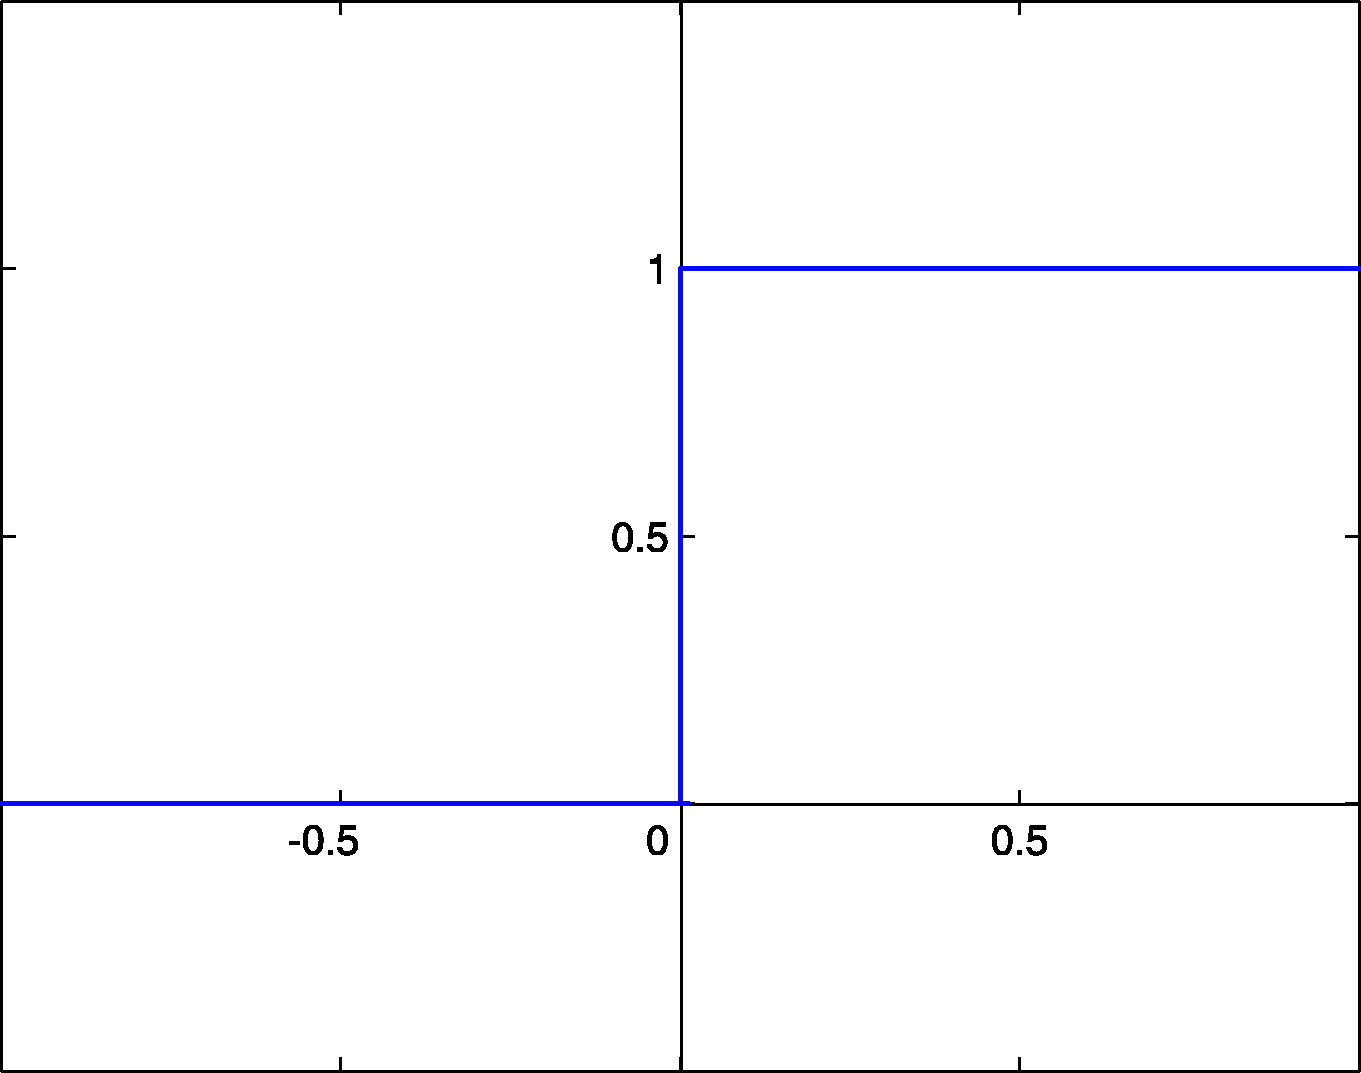
\includegraphics[width=2.8in]{imagens/RNAlimiar.png}}
  \subfigure[Função sigmóide.]{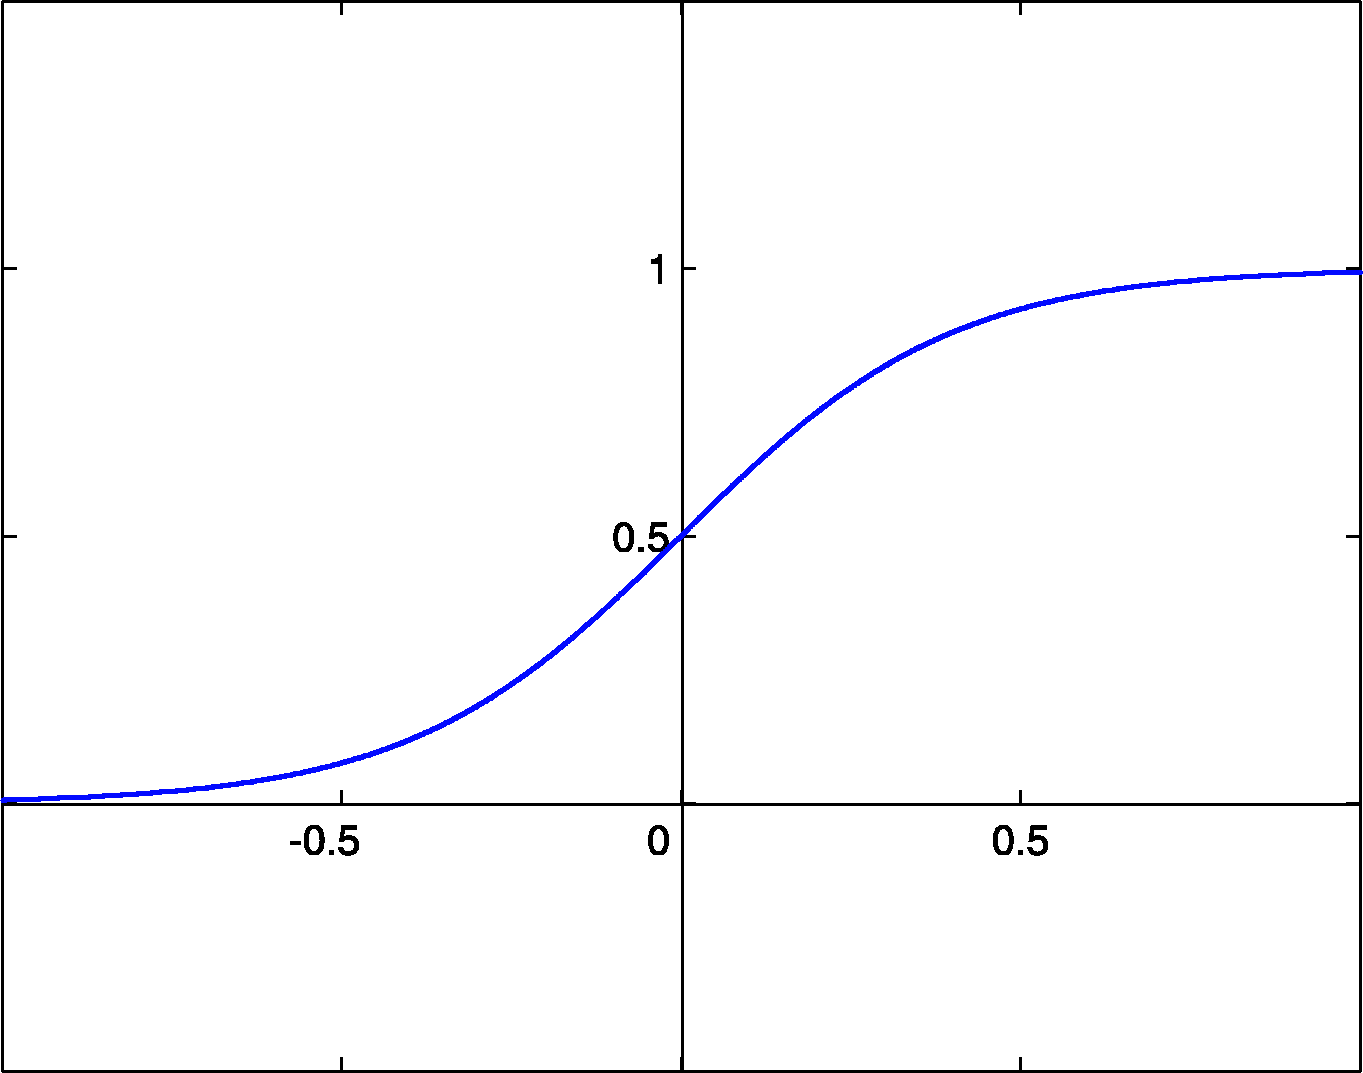
\includegraphics[width=2.8in]{imagens/RNAsigmoide.png}}
 \end{center}
 \caption{Funções de ativação comuns em RNAs.}
 \label{fig:func:rna}
\end{figure}

Na maioria dos casos, será matematicamente conveniente substituir o valor de limiar com um peso extra de entrada no nodo. Dessa forma podemos utilizar um algoritmo mais simples de aprendizado, pois teremos a necessidade de atualizar apenas os pesos, e não os pesos e os limiares. Esse peso extra que deveria ter um valor de ativação vindo de um nodo ou uma entrada, terá sempre $-1$ como valor de ativação. Servindo assim como um limiar $t$, considerando que $w_{0,j} \cdot a_0 = -t$, então todos os nodos poderã ter o limiar fixo em 0.

Existe uma variedade de tipos de estruturas de RNAs, e cada uma resulta em propriedades computacionais muito diferentes. A maior distinção pode ser feita entre as pró-alimentadas e as recorrentes. Nas pró-alimentadas as arestas são unidirecionais e não possuem ciclos, ou seja, são grafos acíclicos direcionados. Numa estrutura recorrente, elas podem formar topologias arbitrárias.

\subsection{Perceptron de múltiplas camadas pró-alimentado}

Um RNA para ser considerada um perceptron de múltiplas camadas deve ter além dos nodos de entrada e saída, nodos intermediários, os quais interagem apenas com outro nodos \cite{sandhya}. Podemos ver um perceptron de múltiplas camadas pró-alimentado na figura \ref{fig:rna}.

% TODO: melhorar imagem.
\begin{figure}[ht]
 \begin{center}
  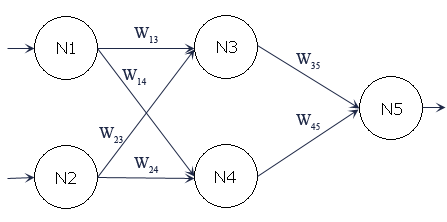
\includegraphics[width=4in]{imagens/rna.png}
 \end{center}
 \caption{Perceptron de múltiplas camadas pró-alimentado simples.}
 \label{fig:rna}
\end{figure}

Com uma camadas de nodos intermediários (suficientemente grande), é possível representar qualquer função contínua das entradas, já com duas camadas intermediárias é possível representar até funções descontínuas.

\subsection{Algoritmo de retro-propagação}

A maneira mais popular de se treinar uma RNA de múltiplas camadas é utilizando o algoritmo de retro-propagação. Ele tenta minimizar o erro entre o valor de saída e o valor esperado, verificando qual é a contribuição de cada peso no erro.

Desta forma, se a RNA calcular um valor correto, os pesos não são alterados. Mas se houver diferença entre o valor esperado e o calculado, os pesos são ajustados de forma a reduzir o erro. Para os nodos de saída utiliza-se a equação \ref{equa:back:output}, $t_j$ é a saída do nodo $j$ e $o_j$ a saída esperada do nodo $j$.

\begin{equation}
	w_{i,j} = w_{i,j} + a \cdot a_i \cdot (t_j - o_j) \cdot g'(e_j)
	\label{equa:back:output}
\end{equation}

Sendo $a$ uma constante chamada de taxa de aprendizado, $e_j$ o resultado da função de entrada e $g'()$ é a derivada da função de ativação. Será conveniente definir $\Delta_j = (t_j - o_j) \cdot g'(e_j)$. A regra de atualização de pesos pode ser escrito como

\begin{equation}
	w_{i,j} = w_{i,j} + a \cdot a_i \cdot \Delta_j
\end{equation}

Para a atualização dos pesos dos nodos de entrada e intermediários nós precisamos definir uma quantidade análoga ao $\Delta_j$ dos nodos de saída. Este ponto é onde a retro-propagação do erro ocorre. Cada nodo $i$ é "responsável" por uma fração do erro $\Delta_j$ em cada um dos nodos de saída em que ele se conecta. Então o valor de $\Delta_j$ é dividido de acordo com a influência da conexão entre o nodo intermediário e o nodo de saída e propagado de volta para que os valores de $\Delta_i$ sejam calculados. A regra de propagação é a seguinte

\begin{equation}
	\Delta_i = g'(e_i) \cdot \sum_j w_{i,j} \cdot \Delta_j
\end{equation}

Agora a equação de atualização dos pesos dos nodos de entrada e intermediários é igual a dos nodos de saída, devemos apenas tomar cuidado no cálculo dos $\Delta$, que são diferentes.

\section{Eficiência de um sistema de CBIR}

As medidas mais usadas para avaliar a qualidado dos resultados de um sistema de CBIR são a precisão e o \textit{recall}, os quais são calculados pelas equações \ref{equa:precisao} e \ref{equa:recall}, respectivamente.

\begin{equation}
	\textit{precisão} = \frac{\textit{número de imagens relevantes recuperadas}}{\textit{número de imagens recuperadas}}
	\label{equa:precisao}
\end{equation}

\begin{equation}
	\textit{precisão} = \frac{\textit{número de imagens relevantes recuperadas}}{\textit{número de imagens relevantes}}
	\label{equa:recall}
\end{equation}

É trivial atingir um \textit{recall} de 100\% retornando todas as imagens do banco. Por isso o \textit{recall} sozinho não é uma medida boa, deve ser interpretada junto a precisão do sistema. Geralmente, existe uma relação inversa entre a precisão e o \textit{recall}, onde é possível aumentar um ao custo de reduzir o outro.
